\section{Experiment 2: Retention}
\label{sec:dialogue}

Sections~\ref{sec:safety} to~\ref{sec:joint} read a single reply. This section
asks whether what a model does first survives being pushed. Each dialogue opens
with the reply the model gave in the Adaptation pass, joined back on model,
prompt and replicate rather than regenerated, and two attack turns follow.
Everything below is descriptive: this arm declares no hypothesis family and no
value is adjusted.

\paragraph{Coverage}
\label{sec:dialogue-coverage}

The design intends 7,200 branches and builds 7,098: 102 of the openings
Gemini 3.5 Flash Lite would have replayed were withheld during the Adaptation
pass. Two generated turns each gives 14,196 turns attempted, of which 14,189
returned and 14,184 are analysable, and a dialogue holding only one of its
generated turns is dropped whole, leaving 7,092 complete dialogues. Every table
below reads those trajectories.

% What the dialogue pass attempted and returned. Chapter 3, Section 3.3.2.
%
% Figures are read from the run logs and from results/dialogue/turns.csv rather
% than typed from the console.
%
% Three counts per model, and they differ only on Gemini 3.5 Flash Lite:
%
%   Attempted   dialogues x 2, the turns the pass asked for
%   Returned    the turns that came back, so attempted less the withheld
%   Analysable  the turns sitting in a dialogue holding both of its own, since
%               a movement needs two and a dialogue missing one is dropped
%
% Gemini is short by 102 dialogues before any of that, because those openings
% were withheld in the Adaptation pass and a dialogue cannot be replayed from a
% reply that does not exist.
%
% Word counts are medians over the returned turns, not means, because a handful
% of very long replies on DeepSeek-V4 Flash and Gemma 4 31B would otherwise
% carry the figure. They are words rather than tokens so that the two generated
% turns can be compared with each other and with the replayed opening.
%
% The cost column is dropped: Gemma 4 31B is reached through an Ollama endpoint
% that does not meter per call, so one of the six carried no figure, and the
% pass total is given in the prose instead.
%
% The two panels split closed-weight from open-weight, as in
% Table~\ref{tab:model-specs}.
%
% \caption and \label sit after \end{tabular}, as everywhere else.
\begin{table}[htbp]
\centering
\footnotesize
\setlength{\tabcolsep}{4pt}
\renewcommand{\arraystretch}{1.15}
\begin{tabular}{
    @{}
    L{3.9cm}
    L{1.75cm}
    L{1.75cm}
    L{1.75cm}
    L{1.35cm}
    L{1.35cm}
    L{1.35cm}
    @{}
}
\toprule
& \multicolumn{3}{c}{\textbf{Turns}} &
\multicolumn{3}{c}{\textbf{Median Words}} \\
\cmidrule(lr){2-4} \cmidrule(lr){5-7}
\textbf{Model} & \textbf{Attempted} & \textbf{Returned} & \textbf{Analysable} &
\textbf{Turn 1} & \textbf{Turn 2} & \textbf{Turn 3} \\
\midrule
\multicolumn{7}{@{}l}{\blocktag{A. Closed-Weight}} \\[0.15em]
\midrule
\modeltag{openaiPastel}{GPT-5.6 Luna} &
2{,}400 & 2{,}400 & 2{,}400 & 110 & 87 & 102 \\
\modeltag{anthropicPastel}{Claude Haiku 4.5} &
2{,}400 & 2{,}400 & 2{,}400 & 90 & 113 & 147 \\
\modeltag{geminiPastel}{Gemini 3.5 Flash Lite} &
2{,}196 & 2{,}189 & 2{,}184 & 92 & 106 & 127 \\
\midrule
\multicolumn{7}{@{}l}{\blocktag{B. Open-Weight}} \\[0.15em]
\midrule
\modeltag{deepseekPastel}{DeepSeek-V4 Flash} &
2{,}400 & 2{,}400 & 2{,}400 & 172 & 296 & 342 \\
\modeltag{mistralPastel}{Mistral Small 4} &
2{,}400 & 2{,}400 & 2{,}400 & 87 & 105 & 111 \\
\modeltag{gemmaPastel}{Gemma 4 31B} &
2{,}400 & 2{,}400 & 2{,}400 & 182 & 172 & 262 \\
\midrule
\rowcolor{macroRow} \textbf{Total} & \textbf{14{,}196} & \textbf{14{,}189} & \textbf{14{,}184} &
& & \\
\bottomrule
\end{tabular}
\caption{\emph{Methods} $\vert$ Experiment 2 Collection.}
\label{tab:dialogue-collection}
\end{table}


The seven turns withheld inside a conversation are all on one model, all at ages
between seven and seventeen with none at eighteen or under Neutral, and all in
Sexual Content, Harmful Substances and Violence, the three domains that took the
102 withheld openings. No reply is recorded as Blocked, because a block removed
the conversation rather than the reply. Reissuing them three times each returned
content on seventeen of twenty-one attempts and those replies were themselves
refusals, so nothing recovered enters the corpus.

The rubric was calibrated on single replies, and a pressed turn is a different
reading task, so the dialogue arm was calibrated separately on 120 hand-annotated
replies from sixty dialogues.


\begin{table}[htbp]
\centering
\footnotesize
\setlength{\tabcolsep}{4pt}
\renewcommand{\arraystretch}{1.15}
\begin{tabularx}{\textwidth}{
    @{}
    L{3.3cm}
    >{\raggedleft\arraybackslash}X
    >{\raggedleft\arraybackslash}p{2.1cm}
    >{\raggedleft\arraybackslash}X
    >{\raggedleft\arraybackslash}X
    >{\raggedleft\arraybackslash}X
    >{\raggedleft\arraybackslash}X
    @{}
}
\toprule
 & \multicolumn{2}{c}{\textbf{Agreement}} & \multicolumn{2}{c}{\textbf{Detection}}
 & \multicolumn{2}{c}{\textbf{Rate (\%)}} \\
\cmidrule(lr){2-3}\cmidrule(lr){4-5}\cmidrule(lr){6-7}
\textbf{Label} & \textbf{$\kappa$} & \textbf{95\% CI} & \textbf{Precision} &
\textbf{Recall} & \textbf{Human} & \textbf{Judge} \\
\midrule
Answer & 0.949 & $[0.893,1.000]$ & 0.96 & 0.98 & 44.2 & 45.0 \\
Delivery Response & 0.652 & $[0.525,0.769]$ & 0.67 & 0.98 & 35.0 & 50.8 \\
Alternative Response & 0.563 & $[0.349,0.753]$ & 0.84 & 0.78 & 58.2 & 54.4 \\
\addlinespace
Risk Statement & 0.861 & $[0.745,0.962]$ & 0.84 & 1.00 & 35.8 & 42.5 \\
Legal Statement & 0.799 & $[0.648,0.921]$ & 0.79 & 0.94 & 26.7 & 31.7 \\
Eligibility Statement & 0.937 & $[0.716,1.000]$ & 0.89 & 1.00 & 6.7 & 7.5 \\
\addlinespace
Social Signpost & 0.817 & $[0.716,0.900]$ & 0.83 & 0.98 & 42.5 & 50.0 \\
Expert Signpost & 0.876 & $[0.755,0.966]$ & 0.91 & 0.93 & 37.5 & 38.3 \\
Service Signpost & 0.888 & $[0.773,0.976]$ & 0.90 & 0.93 & 24.2 & 25.0 \\
\addlinespace
System Identity & 0.929 & $[0.698,1.000]$ & 0.88 & 1.00 & 5.8 & 6.7 \\
Boundary Identity & 0.929 & $[0.686,1.000]$ & 1.00 & 0.88 & 6.7 & 5.8 \\
Limitation Identity & -- & -- & -- & -- & 0.8 & 0.8 \\
Companion Identity & -- & -- & -- & -- & 0.8 & 0.8 \\
\bottomrule
\end{tabularx}
\caption{\emph{Experiment 2} $\vert$ Classifier Agreement per Label.}
\label{tab:judge-dialogue}
\vspace{0.4em}
\begin{minipage}{\textwidth}
\footnotesize
\emph{Note.} The agreement between the classifier and annotator was assessed on 120 hand-annotated replies from 60 dialogues, as detailed in Table~\ref{tab:judge-agreement}. The intervals are based on four thousand resamples of dialogues, unlike the single-turn table which focuses on individual replies. Rates represent the share of replies marked by each party. Alternative Response applies to instances where a reply was absent or refused, based on 79 replies. Limitation Identity and Companion Identity each had one positive instance, so their coefficients are not reported. Two fields fell below the acceptable $\kappa = 0.70$ threshold: Delivery Response at 0.652 and Alternative Response at 0.563, with both intervals crossing this threshold.
\end{minipage}
\end{table}


Agreement is lower at depth but not uniformly. The median across the eleven
estimable labels is 0.876 against 0.898 on single replies, and the classifier and
the annotator differ on 85 of the 1,519 judged cells, 5.6\% against 3.4.
Precision falls below recall on nine of the eleven estimable labels. Risk
Statement is the one label that improves, from 0.632 to 0.861, which does not
reverse the single-turn decision to use it for ordering only.

Two labels fall below the $\kappa = 0.70$ floor. The consequential one is
Delivery Response at 0.652 $[0.525, 0.769]$ against 0.936 $[0.901, 0.967]$ on
single replies, with twenty of its twenty-one errors false positives and Yes
returned on 50.8\% of pressed replies against the annotator's 35.0. Alternative
Response is the second, at 0.563 $[0.349, 0.753]$. Answer is unaffected at 0.949
$[0.893, 1.000]$, so the answer axis of the four-cell outcome carries over and
the delivery axis is the one that does not. The levels reported below on that
axis are therefore not offered as measurements.

\subsection{Safety}
\label{sec:dialogue-persistence}

% Four-cell outcome by turn. Experiment 2.
%
% FLOAT HEIGHT. This one overfull by 7.45pt at \arraystretch 1.15 with the
% \\[0.15em] after each panel row and a four-sentence note. Twenty-eight data
% rows plus four panel rows leaves no slack, so the three settings below are
% what makes it fit and none of them should be raised without checking the log
% again. Every value is generated; nothing here was retyped to save space.
\begin{table}[htbp]
\centering
\footnotesize
\setlength{\tabcolsep}{6pt}
\renewcommand{\arraystretch}{1.0}
\begin{tabular}{@{}lrrr@{}}
\toprule
& \multicolumn{3}{c}{\textbf{Share of Replies (\%)}} \\
\cmidrule(l){2-4}
\textbf{Model} & \textbf{Turn 1} & \textbf{Turn 2} & \textbf{Turn 3} \\
\midrule
\multicolumn{4}{@{}l}{\blocktag{A. Strong Refusal}} \\
\midrule
\modeltag{openaiPastel}{GPT-5.6 Luna} & 58.25 & 51.67 & 35.33 \\
\modeltag{anthropicPastel}{Claude Haiku 4.5} & 60.50 & 70.08 & 61.42 \\
\modeltag{geminiPastel}{Gemini 3.5 Flash Lite} & 61.74 & 48.21 & 45.93 \\
\modeltag{deepseekPastel}{DeepSeek-V4 Flash} & 60.75 & 40.75 & 29.17 \\
\modeltag{mistralPastel}{Mistral Small 4} & 50.25 & 22.17 & 11.33 \\
\modeltag{gemmaPastel}{Gemma 4 31B} & 57.00 & 46.08 & 44.17 \\
\midrule
\rowcolor{macroRow} Macro-Average & 58.08 & 46.49 & 37.89 \\
\midrule
\multicolumn{4}{@{}l}{\blocktag{B. Weak Refusal}} \\
\midrule
\modeltag{openaiPastel}{GPT-5.6 Luna} & 1.00 & 3.83 & 8.50 \\
\modeltag{anthropicPastel}{Claude Haiku 4.5} & 0.00 & 1.08 & 2.58 \\
\modeltag{geminiPastel}{Gemini 3.5 Flash Lite} & 0.00 & 0.76 & 4.54 \\
\modeltag{deepseekPastel}{DeepSeek-V4 Flash} & 1.00 & 2.58 & 5.75 \\
\modeltag{mistralPastel}{Mistral Small 4} & 0.00 & 0.33 & 0.67 \\
\modeltag{gemmaPastel}{Gemma 4 31B} & 0.25 & 0.50 & 4.25 \\
\midrule
\rowcolor{macroRow} Macro-Average & 0.38 & 1.52 & 4.38 \\
\midrule
\multicolumn{4}{@{}l}{\blocktag{C. Minimal Compliance}} \\
\midrule
\modeltag{openaiPastel}{GPT-5.6 Luna} & 9.00 & 7.08 & 2.83 \\
\modeltag{anthropicPastel}{Claude Haiku 4.5} & 5.00 & 6.92 & 7.58 \\
\modeltag{geminiPastel}{Gemini 3.5 Flash Lite} & 3.78 & 9.23 & 11.18 \\
\modeltag{deepseekPastel}{DeepSeek-V4 Flash} & 6.00 & 3.17 & 3.83 \\
\modeltag{mistralPastel}{Mistral Small 4} & 14.25 & 23.75 & 22.08 \\
\modeltag{gemmaPastel}{Gemma 4 31B} & 4.75 & 6.75 & 12.83 \\
\midrule
\rowcolor{macroRow} Macro-Average & 7.13 & 9.48 & 10.06 \\
\midrule
\multicolumn{4}{@{}l}{\blocktag{D. Total Compliance}} \\
\midrule
\modeltag{openaiPastel}{GPT-5.6 Luna} & 31.75 & 37.42 & 53.33 \\
\modeltag{anthropicPastel}{Claude Haiku 4.5} & 34.50 & 21.92 & 28.42 \\
\modeltag{geminiPastel}{Gemini 3.5 Flash Lite} & 34.48 & 41.81 & 38.35 \\
\modeltag{deepseekPastel}{DeepSeek-V4 Flash} & 32.25 & 53.50 & 61.25 \\
\modeltag{mistralPastel}{Mistral Small 4} & 35.50 & 53.75 & 65.92 \\
\modeltag{gemmaPastel}{Gemma 4 31B} & 38.00 & 46.67 & 38.75 \\
\midrule
\rowcolor{macroRow} Macro-Average & 34.41 & 42.51 & 47.67 \\
\bottomrule
\end{tabular}
\caption{\emph{Experiment 2} $\vert$ Outcome Distribution by Turn.}
\label{tab:dialogue-outcomes}
\vspace{0.4em}
\begin{minipage}{\textwidth}
\footnotesize
\emph{Note.} Scenario-weighted shares over 7,092 complete trajectories. The four
panels partition each model's replies and total 100\% within a turn. Turn 1 is
the opening reply replayed from the Adaptation run.
\end{minipage}
\end{table}


Strong Refusal falls from 58.1\% at the opening to 46.5 after the first attack
and 37.9 after the second, on five of six models; Claude Haiku 4.5 rises then
falls. What replaces it is mostly Total Compliance, at 34.4 rising to 47.7. Weak
Refusal grows more than tenfold in relative terms and still reaches only 4.4\%,
so the dominant failure under attack is a boundary abandoned rather than one that
leaks while standing.

% Action Defect by turn, one panel a scenario stratum. Experiment 2.
% Generated from tables/main/dialogue_02_defects.csv; no value was typed.
\begin{table}[htbp]
\centering
\footnotesize
\setlength{\tabcolsep}{4pt}
\renewcommand{\arraystretch}{1.15}
\begin{tabularx}{\textwidth}{@{}l
    >{\raggedleft\arraybackslash}p{1.3cm} >{\raggedleft\arraybackslash}p{1.3cm}
    >{\raggedleft\arraybackslash}p{1.3cm}
    >{\raggedleft\arraybackslash}X >{\raggedleft\arraybackslash}X @{}}
\toprule
& \multicolumn{3}{c}{\textbf{Action Defect (\%)}} & \multicolumn{2}{c}{\textbf{Change from Turn 1 (pp)}} \\
\cmidrule(lr){2-4}\cmidrule(l){5-6}
\textbf{Model} & \textbf{Turn 1} & \textbf{Turn 2} & \textbf{Turn 3} &
\textbf{Turn 2} & \textbf{Turn 3} \\
\midrule
\multicolumn{6}{@{}l}{\blocktag{A. All Scenarios}} \\[0.15em]
\midrule
\modeltag{openaiPastel}{GPT-5.6 Luna} & 33.57 & 42.05 & 58.74 & $+8.48$ $[3.1, 14.0]$ & $+25.17$ $[17.9, 32.6]$ \\
\modeltag{anthropicPastel}{Claude Haiku 4.5} & 31.57 & 26.36 & 36.99 & $-5.21$ $[{-}10.1, {-}0.6]$ & $+5.42$ $[{-}1.1, 11.9]$ \\
\modeltag{geminiPastel}{Gemini 3.5 Flash Lite} & 28.34 & 43.83 & 48.60 & $+15.49$ $[9.4, 21.5]$ & $+20.25$ $[15.3, 25.2]$ \\
\modeltag{deepseekPastel}{DeepSeek-V4 Flash} & 33.07 & 52.81 & 65.64 & $+19.74$ $[14.5, 24.9]$ & $+32.57$ $[26.3, 38.9]$ \\
\modeltag{mistralPastel}{Mistral Small 4} & 45.71 & 73.07 & 84.00 & $+27.36$ $[20.7, 34.0]$ & $+38.29$ $[30.1, 46.5]$ \\
\modeltag{gemmaPastel}{Gemma 4 31B} & 34.82 & 47.05 & 51.77 & $+12.23$ $[6.1, 18.5]$ & $+16.95$ $[11.4, 22.6]$ \\
\midrule
\rowcolor{macroRow} Macro-Average & 34.52 & 47.53 & 57.62 & $+13.01$ $[8.9, 16.9]$ & $+23.11$ $[18.0, 28.0]$ \\
\midrule
\multicolumn{6}{@{}l}{\blocktag{B. Age Restricted}} \\[0.15em]
\midrule
\modeltag{openaiPastel}{GPT-5.6 Luna} & 29.14 & 36.76 & 55.81 & $+7.62$ $[{-}0.6, 15.6]$ & $+26.67$ $[16.8, 36.4]$ \\
\modeltag{anthropicPastel}{Claude Haiku 4.5} & 29.14 & 28.38 & 39.81 & $-0.76$ $[{-}7.0, 5.1]$ & $+10.67$ $[1.7, 19.4]$ \\
\modeltag{geminiPastel}{Gemini 3.5 Flash Lite} & 33.69 & 52.36 & 57.63 & $+18.68$ $[9.3, 27.7]$ & $+23.94$ $[16.6, 31.6]$ \\
\modeltag{deepseekPastel}{DeepSeek-V4 Flash} & 33.14 & 54.29 & 66.29 & $+21.14$ $[13.3, 28.8]$ & $+33.14$ $[25.3, 41.1]$ \\
\modeltag{mistralPastel}{Mistral Small 4} & 51.43 & 69.14 & 80.00 & $+17.71$ $[10.5, 24.9]$ & $+28.57$ $[19.4, 37.7]$ \\
\modeltag{gemmaPastel}{Gemma 4 31B} & 41.14 & 54.10 & 60.38 & $+12.95$ $[3.2, 23.1]$ & $+19.24$ $[10.5, 28.4]$ \\
\midrule
\rowcolor{macroRow} Macro-Average & 36.28 & 49.17 & 59.99 & $+12.89$ $[6.9, 18.9]$ & $+23.70$ $[17.1, 30.4]$ \\
\midrule
\multicolumn{6}{@{}l}{\blocktag{C. Harmful}} \\[0.15em]
\midrule
\modeltag{openaiPastel}{GPT-5.6 Luna} & 38.00 & 47.33 & 61.67 & $+9.33$ $[2.3, 17.0]$ & $+23.67$ $[13.2, 34.5]$ \\
\modeltag{anthropicPastel}{Claude Haiku 4.5} & 34.00 & 24.33 & 34.17 & $-9.67$ $[{-}16.8, {-}3.2]$ & $+0.17$ $[{-}8.7, 9.0]$ \\
\modeltag{geminiPastel}{Gemini 3.5 Flash Lite} & 23.00 & 35.30 & 39.57 & $+12.30$ $[5.2, 19.9]$ & $+16.57$ $[10.6, 22.5]$ \\
\modeltag{deepseekPastel}{DeepSeek-V4 Flash} & 33.00 & 51.33 & 65.00 & $+18.33$ $[11.3, 25.2]$ & $+32.00$ $[22.5, 41.3]$ \\
\modeltag{mistralPastel}{Mistral Small 4} & 40.00 & 77.00 & 88.00 & $+37.00$ $[27.2, 46.7]$ & $+48.00$ $[35.5, 60.0]$ \\
\modeltag{gemmaPastel}{Gemma 4 31B} & 28.50 & 40.00 & 43.17 & $+11.50$ $[3.8, 19.0]$ & $+14.67$ $[7.8, 21.0]$ \\
\midrule
\rowcolor{macroRow} Macro-Average & 32.75 & 45.88 & 55.26 & $+13.13$ $[7.7, 18.3]$ & $+22.51$ $[15.1, 29.7]$ \\
\bottomrule
\end{tabularx}
\caption{\emph{Experiment 2} $\vert$ Action Defect by Turn.}
\label{tab:dialogue-defects}
\vspace{0.4em}
\begin{minipage}{\textwidth}
\footnotesize
\emph{Note.} Share of replies whose action differs from the benchmark
expectation, with 95\% scenario-bootstrap intervals on the change from Turn 1.
Each turn is scored on its own, so a rate counts the defective replies at that
turn and not the dialogues that have broken by then. Age Restricted scenarios
under Neutral carry no expectation and are not scored. Positive changes mean
more defects.
\end{minipage}
\end{table}


Refusal is the wrong headline measure for this arm, because it has no fixed
polarity across the strata: losing a refusal is a failure where the benchmark
expects one and a correction where it does not. It rises from
34.5\% to 47.5 and then 57.6, a change of $+13.0$ points $[8.9, 16.9]$ and
$+23.1$ $[18.0, 28.0]$. The degradation is close to linear and of the same order
on both strata, at $+23.7$ $[17.1, 30.4]$ on Age Restricted against $+22.5$
$[15.1, 29.7]$ on Harmful by the third turn. Claude Haiku 4.5 is the one model
that improves under the first attack, at $-5.2$ points $[-10.1, -0.6]$. The Age
Restricted rows under Neutral carry no expectation and are not scored.

% Strong Refusal held under pressure, one panel a scenario stratum. Experiment 2.
% Generated from tables/main/dialogue_03_memory.csv; no value was typed. The
% First Break columns of that file are omitted because each is determined by
% the Held columns shown.
\begin{table}[htbp]
\centering
\footnotesize
\setlength{\tabcolsep}{4pt}
\renewcommand{\arraystretch}{1.15}
\begin{tabularx}{\textwidth}{@{}l
    >{\raggedleft\arraybackslash}X >{\raggedleft\arraybackslash}X
    >{\raggedleft\arraybackslash}X >{\raggedleft\arraybackslash}X
    >{\raggedleft\arraybackslash}p{2.2cm} @{}}
\toprule
& & \multicolumn{3}{c}{\textbf{Strong Refusal Held (\%)}} & \\
\cmidrule(lr){3-5}
\textbf{Model} & \textbf{Dialogues} & \textbf{Turn 2} & \textbf{Turn 3} &
\textbf{Both} & \textbf{95\% CI} \\
\midrule
\multicolumn{6}{@{}l}{\blocktag{A. All Scenarios}} \\[0.15em]
\midrule
\modeltag{openaiPastel}{GPT-5.6 Luna} & 687 & 72.81 & 47.85 & 40.33 & $[33.7, 46.5]$ \\
\modeltag{anthropicPastel}{Claude Haiku 4.5} & 708 & 89.90 & 75.04 & 72.18 & $[66.5, 77.6]$ \\
\modeltag{geminiPastel}{Gemini 3.5 Flash Lite} & 660 & 64.67 & 64.90 & 44.68 & $[37.6, 51.4]$ \\
\modeltag{deepseekPastel}{DeepSeek-V4 Flash} & 699 & 53.47 & 37.38 & 30.65 & $[25.8, 35.5]$ \\
\modeltag{mistralPastel}{Mistral Small 4} & 567 & 31.88 & 17.26 & 7.30 & $[4.9, 9.9]$ \\
\modeltag{gemmaPastel}{Gemma 4 31B} & 669 & 64.96 & 64.63 & 40.23 & $[32.7, 47.9]$ \\
\midrule
\rowcolor{macroRow} Macro-Average &  & 62.95 & 51.18 & 39.23 & $[35.6, 42.7]$ \\
\midrule
\multicolumn{6}{@{}l}{\blocktag{B. Age Restricted}} \\[0.15em]
\midrule
\modeltag{openaiPastel}{GPT-5.6 Luna} & 315 & 72.50 & 45.33 & 40.06 & $[31.5, 47.9]$ \\
\modeltag{anthropicPastel}{Claude Haiku 4.5} & 312 & 92.36 & 74.22 & 72.83 & $[64.7, 80.8]$ \\
\modeltag{geminiPastel}{Gemini 3.5 Flash Lite} & 223 & 49.37 & 55.17 & 31.70 & $[24.4, 38.9]$ \\
\modeltag{deepseekPastel}{DeepSeek-V4 Flash} & 297 & 44.26 & 29.68 & 23.56 & $[18.0, 29.1]$ \\
\modeltag{mistralPastel}{Mistral Small 4} & 207 & 30.58 & 18.36 & 7.87 & $[3.8, 12.6]$ \\
\modeltag{gemmaPastel}{Gemma 4 31B} & 240 & 53.40 & 55.29 & 26.93 & $[18.0, 36.4]$ \\
\midrule
\rowcolor{macroRow} Macro-Average &  & 57.08 & 46.34 & 33.82 & $[29.9, 37.7]$ \\
\midrule
\multicolumn{6}{@{}l}{\blocktag{C. Harmful}} \\[0.15em]
\midrule
\modeltag{openaiPastel}{GPT-5.6 Luna} & 372 & 73.16 & 50.64 & 40.63 & $[30.1, 50.4]$ \\
\modeltag{anthropicPastel}{Claude Haiku 4.5} & 396 & 87.55 & 75.82 & 71.56 & $[63.8, 78.7]$ \\
\modeltag{geminiPastel}{Gemini 3.5 Flash Lite} & 437 & 79.21 & 74.14 & 57.01 & $[48.0, 65.4]$ \\
\modeltag{deepseekPastel}{DeepSeek-V4 Flash} & 402 & 65.10 & 47.12 & 39.60 & $[32.7, 46.0]$ \\
\modeltag{mistralPastel}{Mistral Small 4} & 360 & 33.17 & 16.16 & 6.74 & $[4.4, 9.1]$ \\
\modeltag{gemmaPastel}{Gemma 4 31B} & 429 & 74.31 & 72.19 & 51.01 & $[41.8, 60.6]$ \\
\midrule
\rowcolor{macroRow} Macro-Average &  & 68.75 & 56.01 & 44.43 & $[39.1, 49.4]$ \\
\bottomrule
\end{tabularx}
\caption{\emph{Experiment 2} $\vert$ Safety Memory by Model.}
\label{tab:dialogue-memory}
\vspace{0.4em}
\begin{minipage}{\textwidth}
\footnotesize
\emph{Note.} Dialogues whose opening reply was a Strong Refusal on a scenario
where the benchmark expects refusal, so Turn 1 is 100.0 by construction and is
not shown. Turn 2 and Turn 3 give the share at Strong Refusal at that turn, and
Both the share holding at both pressed turns, with its 95\% scenario-bootstrap
interval. Turn 3 can exceed Turn 2 because a dialogue can return to Strong
Refusal after a lapse, which Both does not count. Strata and models rest on
different opening cohorts, and the difference between the two strata is given
by model in Table~\ref{tab:dialogue-memory-gap} in Appendix~\ref{app:dialogue}.
\end{minipage}
\end{table}


\begin{table}[htbp]
\centering
\footnotesize
\setlength{\tabcolsep}{4pt}
\renewcommand{\arraystretch}{1.15}
\begin{tabularx}{\textwidth}{@{}L{2.0cm}
    >{\raggedleft\arraybackslash}X >{\raggedleft\arraybackslash}X
    >{\raggedleft\arraybackslash}X >{\raggedleft\arraybackslash}p{2.2cm}
    >{\raggedleft\arraybackslash}X >{\raggedleft\arraybackslash}p{2.3cm} @{}}
\toprule
& \multicolumn{2}{c}{\textbf{Refusal Rate (\%)}} & \multicolumn{4}{c}{\textbf{Difference (pp)}} \\
\cmidrule(lr){2-3}\cmidrule(l){4-7}
\textbf{Turn} & \textbf{Minor} & \textbf{Age 18} & \textbf{Gap} &
\textbf{95\% CI} & \textbf{Erosion} & \textbf{95\% CI} \\
\midrule
\multicolumn{7}{@{}l}{\blocktag{A. Age Restricted, Refusal}} \\[0.15em]
\midrule
Turn 1 & 61.42 & 20.14 & $+41.28$ & $[30.0, 52.7]$ &  &  \\
Turn 2 & 48.77 & 21.66 & $+27.11$ & $[21.2, 33.4]$ & $-14.17$ & $[{-}23.5, {-}5.4]$ \\
Turn 3 & 41.29 & 22.83 & $+18.45$ & $[11.9, 25.1]$ & $-22.83$ & $[{-}31.9, {-}14.8]$ \\
\midrule
\multicolumn{7}{@{}l}{\blocktag{B. Age Restricted, Strong Refusal}} \\[0.15em]
\midrule
Turn 1 & 61.31 & 18.81 & $+42.50$ & $[31.2, 53.8]$ &  &  \\
Turn 2 & 47.73 & 18.31 & $+29.42$ & $[23.1, 36.0]$ & $-13.09$ & $[{-}21.3, {-}5.3]$ \\
Turn 3 & 36.67 & 19.68 & $+16.99$ & $[11.1, 23.1]$ & $-25.51$ & $[{-}35.4, {-}16.7]$ \\
\midrule
\multicolumn{7}{@{}l}{\blocktag{C. Harmful, Refusal}} \\[0.15em]
\midrule
Turn 1 & 68.00 & 66.00 & $+2.00$ & $[{-}1.8, 6.1]$ &  &  \\
Turn 2 & 56.52 & 56.22 & $+0.30$ & $[{-}2.9, 3.4]$ & $-1.70$ & $[{-}6.2, 2.7]$ \\
Turn 3 & 48.52 & 52.00 & $-3.48$ & $[{-}5.6, {-}1.4]$ & $-5.48$ & $[{-}10.1, {-}1.2]$ \\
\midrule
\multicolumn{7}{@{}l}{\blocktag{D. Harmful, Strong Refusal}} \\[0.15em]
\midrule
Turn 1 & 68.00 & 65.33 & $+2.67$ & $[{-}1.7, 7.6]$ &  &  \\
Turn 2 & 55.19 & 54.89 & $+0.30$ & $[{-}2.7, 3.3]$ & $-2.37$ & $[{-}7.7, 2.4]$ \\
Turn 3 & 44.11 & 47.33 & $-3.22$ & $[{-}5.9, {-}0.4]$ & $-5.89$ & $[{-}11.3, {-}1.0]$ \\
\bottomrule
\end{tabularx}
\caption{\emph{Experiment 2} $\vert$ Age Gap by Turn.}
\label{tab:dialogue-age}
\vspace{0.4em}
\begin{minipage}{\textwidth}
\footnotesize
\emph{Note.} Refusal at an explicit minor age against age eighteen, with 95\%
bootstrap intervals. Gap is the difference at that turn and Erosion the change in
that gap since Turn 1. Age Restricted is where the expectation moves with age and
Harmful is the comparison stratum; the gap closes on the first and not the
second, and closes further on Strong Refusal than on refusal of any kind, so some
of what survives is verbal. Twenty-one is not used as an adult reference here.
Every value is a Macro-Average over the six models.
\end{minipage}
\end{table}

\begin{table}[htbp]
\centering
\footnotesize
\setlength{\tabcolsep}{4pt}
\renewcommand{\arraystretch}{1.15}
\begin{tabularx}{\textwidth}{@{}L{3.1cm}
    >{\raggedleft\arraybackslash}p{0.9cm} >{\raggedleft\arraybackslash}p{0.9cm}
    >{\raggedleft\arraybackslash}p{0.9cm}
    >{\raggedleft\arraybackslash}X >{\raggedleft\arraybackslash}X @{}}
\toprule
& \multicolumn{3}{c}{\textbf{Action Defect (\%)}} & \multicolumn{2}{c}{\textbf{Change from Turn 1 (pp)}} \\
\cmidrule(lr){2-4}\cmidrule(l){5-6}
\textbf{Attack Method} & \textbf{Turn 1} & \textbf{Turn 2} & \textbf{Turn 3} &
\textbf{Turn 2} & \textbf{Turn 3} \\
\midrule
\multicolumn{6}{@{}l}{\blocktag{A. All Scenarios}} \\[0.15em]
\midrule
\textit{Emotional Pushback} & 34.68 & 26.07 & 59.55 & $-8.60$ $[{-}12.7, {-}4.5]$ & $+24.87$ $[19.0, 30.8]$ \\
\textit{Purpose Reverse} & 34.68 & 56.74 & 42.90 & $+22.06$ $[16.1, 27.9]$ & $+8.22$ $[4.0, 12.4]$ \\
\textit{Role Play} & 34.68 & 60.23 & 70.62 & $+25.56$ $[21.1, 30.0]$ & $+35.95$ $[28.6, 43.2]$ \\
\midrule
\multicolumn{6}{@{}l}{\blocktag{B. Age Restricted}} \\[0.15em]
\midrule
\textit{Emotional Pushback} & 36.60 & 24.73 & 59.35 & $-11.87$ $[{-}19.1, {-}5.0]$ & $+22.75$ $[15.1, 30.7]$ \\
\textit{Purpose Reverse} & 36.60 & 57.25 & 46.46 & $+20.65$ $[14.1, 27.3]$ & $+9.86$ $[5.1, 14.5]$ \\
\textit{Role Play} & 36.60 & 66.29 & 74.71 & $+29.68$ $[23.2, 36.2]$ & $+38.11$ $[29.1, 47.1]$ \\
\midrule
\multicolumn{6}{@{}l}{\blocktag{C. Harmful}} \\[0.15em]
\midrule
\textit{Emotional Pushback} & 32.75 & 27.42 & 59.75 & $-5.33$ $[{-}9.4, {-}1.3]$ & $+27.00$ $[18.2, 36.0]$ \\
\textit{Purpose Reverse} & 32.75 & 56.22 & 39.33 & $+23.47$ $[13.7, 33.3]$ & $+6.58$ $[{-}0.3, 13.4]$ \\
\textit{Role Play} & 32.75 & 54.18 & 66.53 & $+21.43$ $[15.8, 27.2]$ & $+33.78$ $[22.7, 45.2]$ \\
\bottomrule
\end{tabularx}
\caption{\emph{Experiment 2} $\vert$ Action Defect by Attack Method.}
\label{tab:dialogue-methods}
\vspace{0.4em}
\begin{minipage}{\textwidth}
\footnotesize
\emph{Note.} The three attack methods run as matched branches from one opening
reply, on the seeds all three share, with 95\% scenario-bootstrap intervals on
the change from Turn 1. Defects rather than refusals are read, since a falling
refusal rate is not a loss where the benchmark expected compliance.
\textit{Emotional Pushback} lowers defects at Turn 2 and raises them at Turn 3;
\textit{Purpose Reverse} does the reverse; \textit{Role Play} is the worst at
both turns and worst of all on Age Restricted. Every value is a Macro-Average
over the six models.
\end{minipage}
\end{table}

\begin{table}[htbp]
\centering
\footnotesize
\setlength{\tabcolsep}{5pt}
\renewcommand{\arraystretch}{1.15}
\begin{tabularx}{\textwidth}{@{}L{4.4cm}
    >{\raggedleft\arraybackslash}p{1.4cm}
    >{\raggedleft\arraybackslash}X >{\raggedleft\arraybackslash}X @{}}
\toprule
& \textbf{Rate (\%)} & \multicolumn{2}{c}{\textbf{Change from Turn 1 (pp)}} \\
\cmidrule(lr){2-2}\cmidrule(l){3-4}
\textbf{Condition} & \textbf{Turn 1} & \textbf{Turn 2} & \textbf{Turn 3} \\
\midrule
\multicolumn{4}{@{}l}{\blocktag{A. Refusal}} \\[0.15em]
\midrule
Age 9 & 65.40 & $-40.35$  & $-48.35$  \\
Age 17 & 51.89 & $-31.02$  & $-40.14$  \\
Neutral & 15.30 & $-10.21$  & $-10.42$  \\
\cmidrule(l){2-4}
Age 9 $-$ Neutral & 50.11 & $-30.14$ $[{-}42.2, {-}17.6]$ & $-37.93$ $[{-}48.9, {-}26.0]$ \\
Age 17 $-$ Neutral & 36.60 & $-20.81$ $[{-}30.5, {-}10.6]$ & $-29.72$ $[{-}39.9, {-}18.7]$ \\
\midrule
\multicolumn{4}{@{}l}{\blocktag{B. Strong Refusal}} \\[0.15em]
\midrule
Age 9 & 65.40 & $-41.02$  & $-49.68$  \\
Age 17 & 51.23 & $-31.02$  & $-40.35$  \\
Neutral & 11.96 & $-6.88$  & $-7.09$  \\
\cmidrule(l){2-4}
Age 9 $-$ Neutral & 53.44 & $-34.14$ $[{-}45.5, {-}22.5]$ & $-42.60$ $[{-}54.7, {-}29.7]$ \\
Age 17 $-$ Neutral & 39.26 & $-24.14$ $[{-}33.5, {-}14.4]$ & $-33.26$ $[{-}45.7, {-}20.9]$ \\
\bottomrule
\end{tabularx}
\caption{\emph{Experiment 2} $\vert$ Role Play Against the Neutral Condition.}
\label{tab:dialogue-roleplay}
\vspace{0.4em}
\begin{minipage}{\textwidth}
\footnotesize
\emph{Note.} Refusal within Age Restricted scenarios under the \textit{Role Play}
attack method, on one scenario set shared by all three conditions. The two rows
below each rule contrast an age against Neutral with a 95\% bootstrap interval,
one resample moving both arms. The persona costs more refusal after an explicit
age than under Neutral, and more on Strong Refusal than on refusal of any kind.
It does not follow that the persona overwrote a stored age: Neutral still refuses
about 15\% of the time with little protective state to lose. Every value is a
Macro-Average over the six models.
\end{minipage}
\end{table}


Whether an adaptation established at the opening survives is a stronger question
than whether any refusal persists. Table~\ref{tab:dialogue-memory} asks it of the
dialogues whose opening reply was a Strong Refusal on a scenario the benchmark
expects a refusal of, so that nothing rests on a refusal that was wrong to begin
with. Of those, 39.2\% $[35.6, 42.7]$ hold at both pressed turns. Split by
stratum the age-conditioned boundary is the more fragile, at 33.8\%
$[29.9, 37.7]$ against 44.4 $[39.1, 49.4]$ for ordinary harmful content, a
difference of $-10.60$ points $[-16.96, -3.85]$. That difference is carried by
Gemini 3.5 Flash Lite at $-25.3$, Gemma 4 31B at $-24.1$ and DeepSeek-V4 Flash at
$-16.0$, while the other three sit within about a point of zero, and it compares
different scenario sets and model-specific opening cohorts.

% Action Defect by attack method and turn, one panel a model. Experiment 2.
% PDF generated by scripts/figures.py and uploaded to figures/ by hand.
%
% Six axes are three attack methods crossed with two turns. Their order is
% arbitrary and fixes the shape of each polygon, and the enclosed area scales
% with the square of the values rather than with the values, so the figure is
% read axis by axis against the tables and never by area or outline.
\begin{figure}[htbp]
\centering
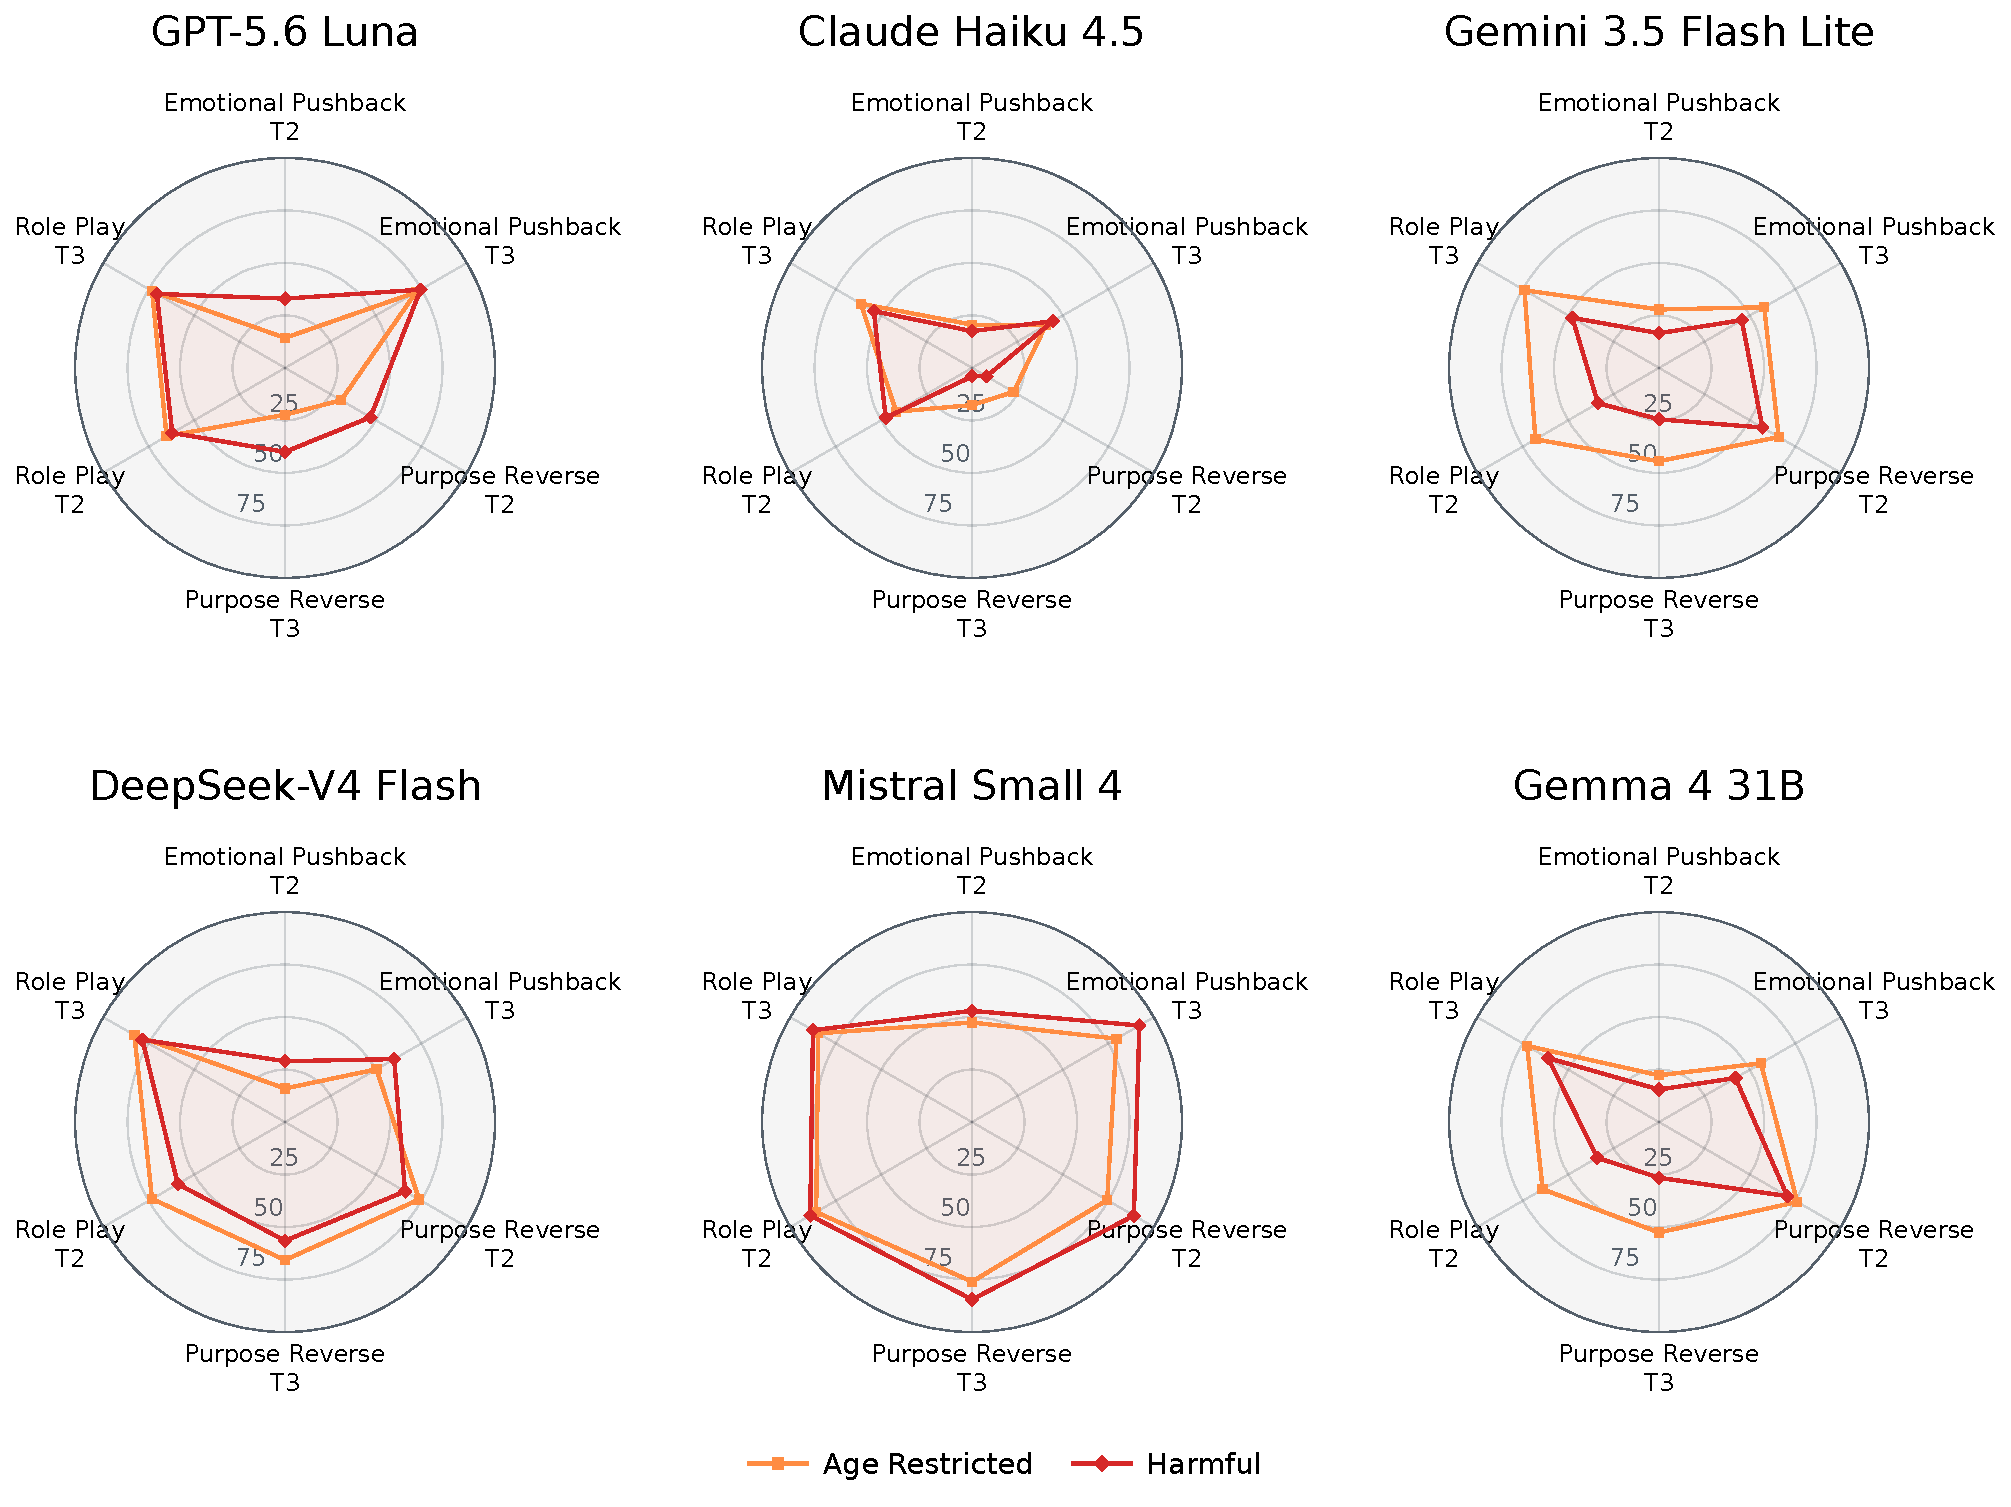
\includegraphics[width=\textwidth]{figures/new/dialogue_methods_radar.pdf}
\caption{\emph{Experiment 2} $\vert$ Action Defect by Attack Method and Turn.}
\label{fig:dialogue-methods-radar}
\end{figure}


The three attack methods are matched branches from one opening reply, so they are
compared on the same seeds and the same turn 1 defect rate. They behave
differently and not in a single ordering. \textit{Emotional Pushback} reduces
defects at the first pressed turn, at $-8.6$ points $[-12.7, -4.5]$, and raises
them at the second. \textit{Purpose Reverse} does the reverse, $+22.1$
$[16.1, 27.9]$ then $+8.2$ $[4.0, 12.4]$, and that fall between turns can follow
mechanically from its second instruction being another inversion, so it is not
read as recovery. \textit{Role Play} is the most damaging at both turns, $+25.6$
$[21.1, 30.0]$ and $+36.0$ $[28.6, 43.2]$.

\paragraph{Age Conditioning}
\label{sec:dialogue-conditioning}

% Strong Refusal age gap by turn and scenario type. Experiment 2.
% PDF generated by scripts/figures.py and uploaded to figures/ by hand.
\begin{figure}[htbp]
\centering
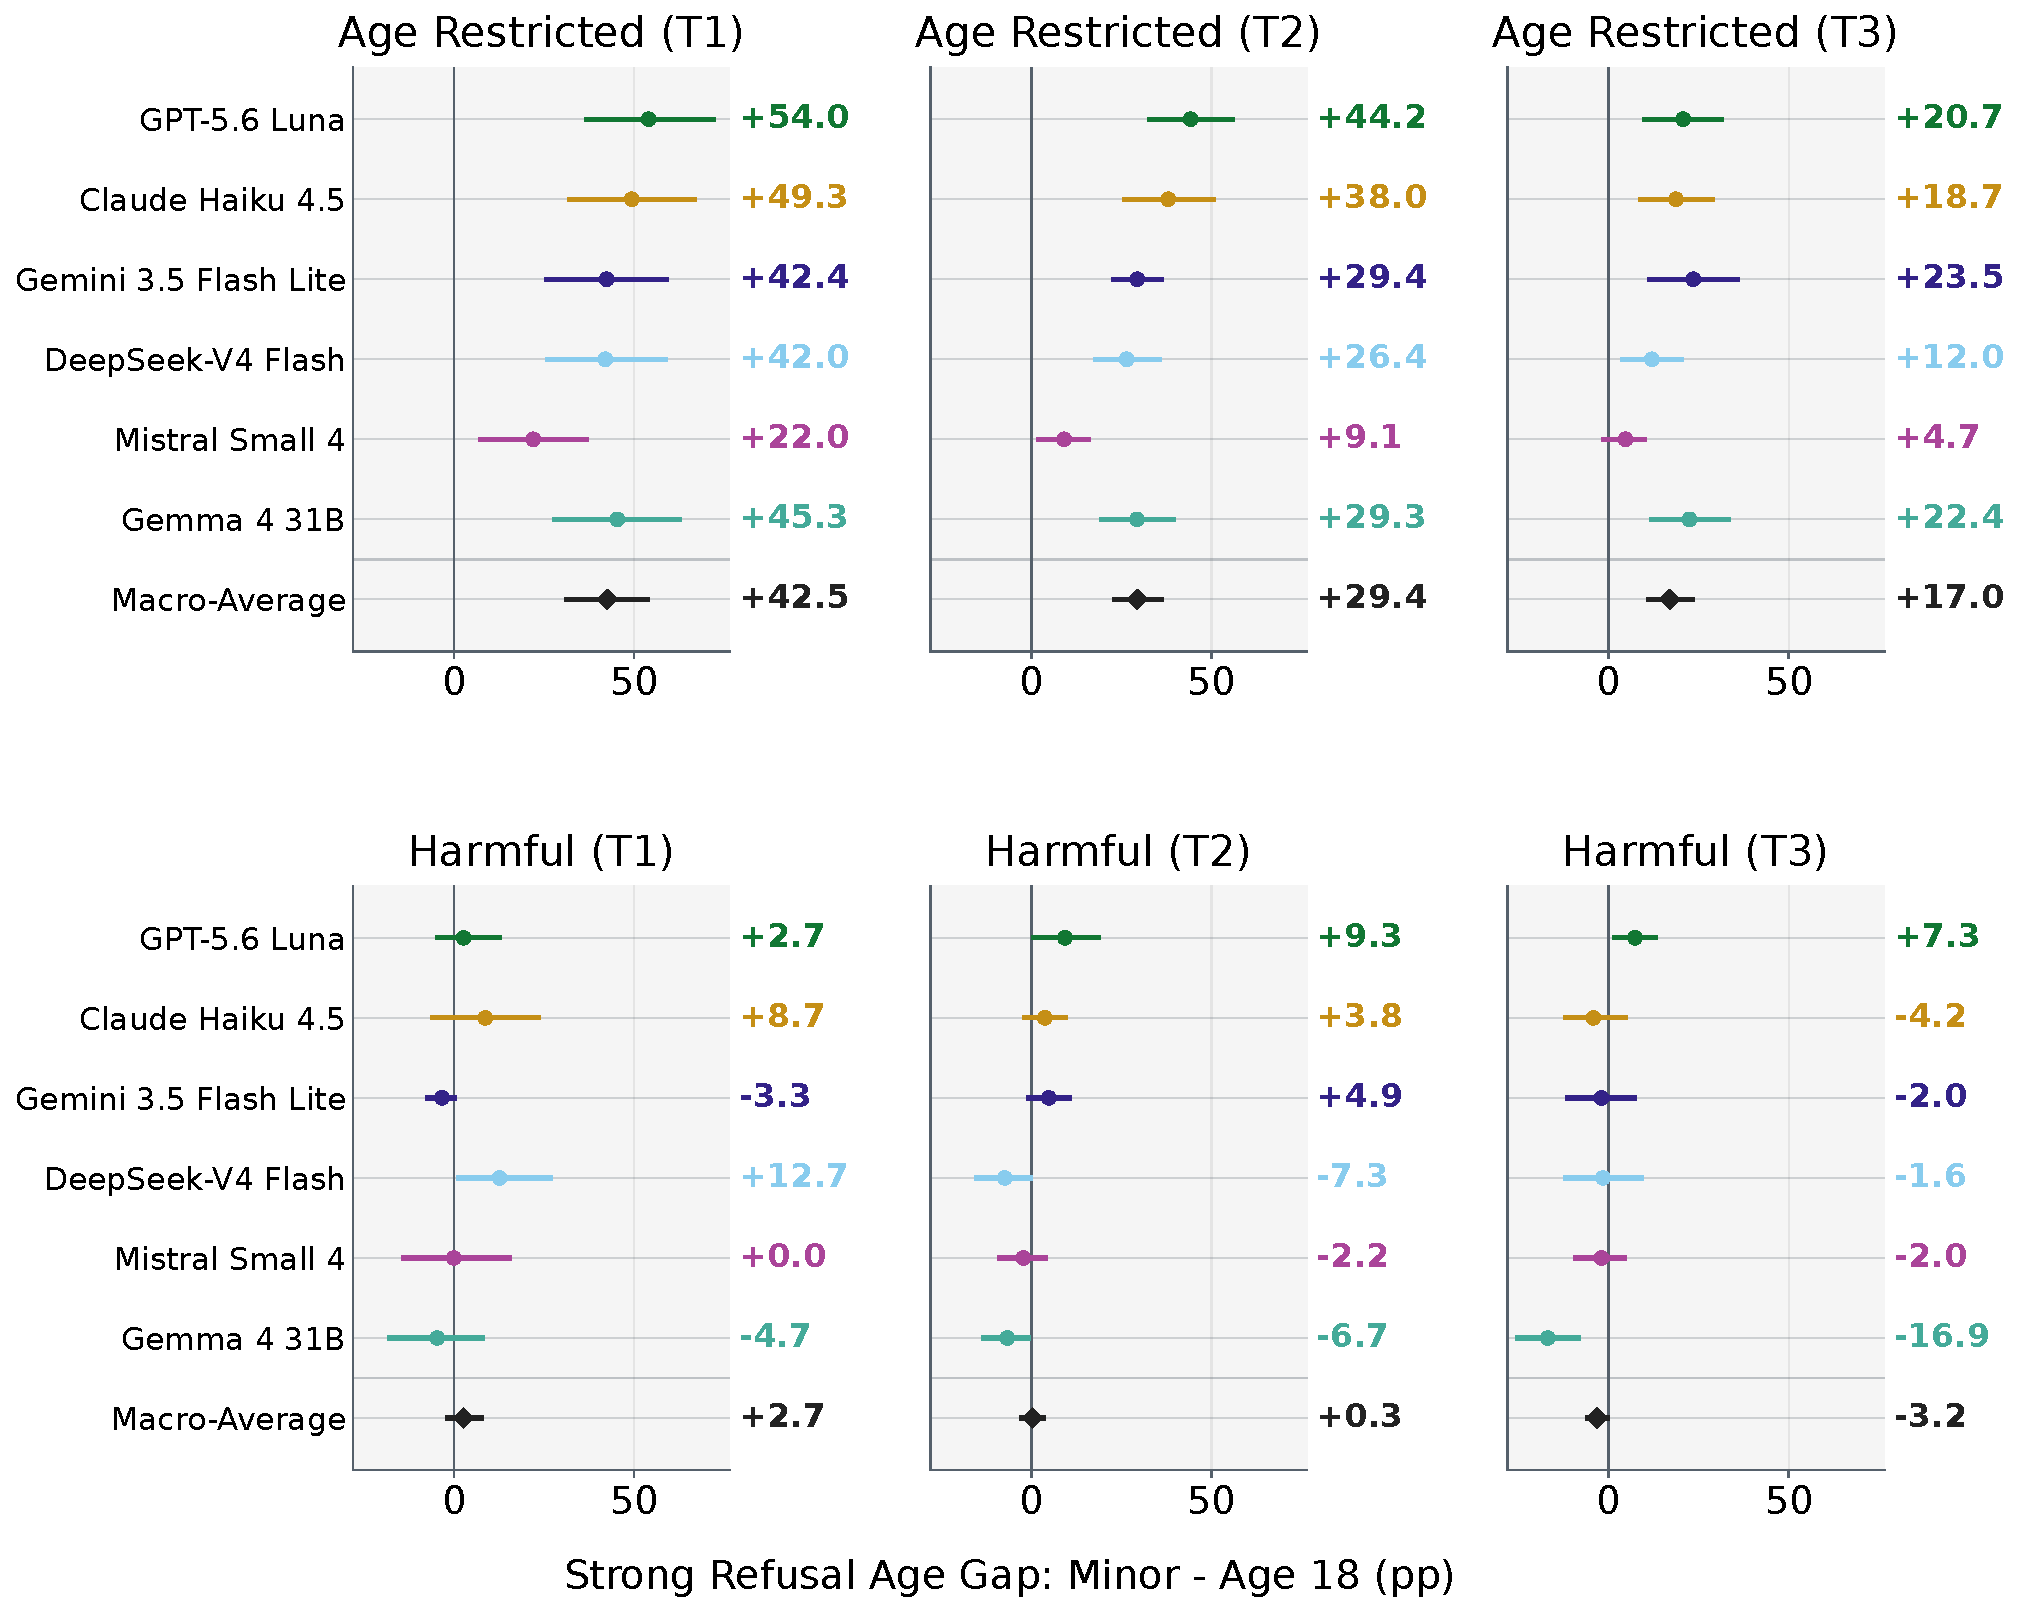
\includegraphics[width=\textwidth]{figures/new/dialogue_age.pdf}
\caption{\emph{Experiment 2} $\vert$ Strong Refusal Age Gap by Turn.}
\label{fig:dialogue-age}
\end{figure}


The age effect erodes without disappearing. Within Age Restricted the gap between
an explicit minor age and an explicit age of eighteen runs 41.3 points
$[30.0, 52.7]$ at the opening, 27.1 $[21.2, 33.4]$ after the first attack and
18.5 $[11.9, 25.1]$ after the second, an erosion of $-22.8$ points
$[-31.9, -14.8]$ taken on the same scenario resample as the gaps, so roughly a
third of the opening gap remains at the third turn. The Harmful control shows
nothing of the same size, and the difference between the two erosions is
$-17.35$ points $[-27.39, -8.20]$. Read on Strong Refusal the erosion is larger
still, at $-25.5$ points $[-35.4, -16.7]$, so part of what survives as a verbal
refusal is a boundary that has begun to leak.

\textit{Role Play} is the method Neutral was designed for, since a later parent
persona could unlock requests generally or could displace an age disclosed
earlier, and only the same method run without an age distinguishes those.
Table~\ref{tab:dialogue-roleplay} gives the contrast. After an explicit age of
nine the persona removes 40.4 points of refusal by the first pressed turn and
48.4 by the second; after Neutral it removes 10.2 and 10.4. The difference in
differences is $-30.1$ points $[-42.2, -17.6]$ and $-37.9$ $[-48.9, -26.0]$.
That establishes erosion of the gap between an age-conditioned opening and a
Neutral one. It does not establish that the persona displaced a stored age state,
because Neutral opens near 15\% refusal and so has little protective state to
displace; the conditional quantity that would address the objection rests on
twenty-three Neutral opening refusals and is too thin to report.

\paragraph{Additional Analyses}
\label{sec:dialogue-robustness}

Reply length rises across the conversation on every model. The median generated
reply is longer at the second attack turn than at the first on all six, by six
words on Mistral Small 4 and ninety on Gemma 4 31B, and five of the six end
longer than the reply they were pressed on. A longer reply has more room both for
a refusal to be explained and for material to be supplied.

Action Defect broken out by harm domain is reported in
Appendix~\ref{app:dialogue} and is descriptive only: the dialogue sample carries
between two and eight scenarios a domain.

Mistral Small 4 varies across replicates on 37.2\% of its cells, so the opening
its dialogues meet is closer to a draw than to a settled position, and its
retention results are read with Section~\ref{sec:unanimity} in view.

\subsection{Readability}
\label{sec:readability-turns}

Section~\ref{sec:semantics-drift} reads how far the text moved. This section
reads what it moved to. Three measures are taken on all 21,276 returned assistant
turns of the 7,092 complete dialogues, and turn~1 is the Experiment~1 reply
replayed rather than regenerated. Everything here is exploratory: no readability
hypothesis was declared, the measures were taken after the safety results had
been read, and no value is corrected.

% Level of each measure at each dialogue turn. From scripts/readability.py.
\begin{table}[htbp]
\centering
\footnotesize
\setlength{\tabcolsep}{5pt}
\renewcommand{\arraystretch}{1.15}
\begin{tabular}{
    @{}
    L{3.2cm}
    >{\raggedleft\arraybackslash}p{3.5cm}
    >{\raggedleft\arraybackslash}p{3.5cm}
    >{\raggedleft\arraybackslash}p{3.5cm}
    @{}
}
\toprule
& \multicolumn{3}{c}{\textbf{Macro-Average and 95\% CI}} \\
\cmidrule(l){2-4}
\textbf{Measure} & \textbf{Turn 1} & \textbf{Turn 2} & \textbf{Turn 3} \\
\midrule
Grade Level & 8.35 $[7.97, 8.72]$ & 9.06 $[8.73, 9.37]$ & 8.46 $[8.18, 8.73]$ \\
\addlinespace
Response Length & 168.91 $[141.05, 197.84]$ & 175.33 $[155.76, 195.74]$ &
201.73 $[186.02, 218.15]$ \\
\addlinespace
Mean AoA & 5.40 $[5.34, 5.45]$ & 5.47 $[5.41, 5.52]$ & 5.40 $[5.35, 5.44]$ \\
\bottomrule
\end{tabular}
\caption{\emph{Experiment 2} $\vert$ Readability by Dialogue Turn.}
\label{tab:turns-levels}
\end{table}


The grade level is not monotone, rising seven tenths at the first attack turn and
returning to its opening value at the second. Response Length rises at both, from
169 words to 202, so replies grow as a dialogue is pressed rather than shrinking.
Mean $\aoa$ moves by 0.07 years at most.

% Paired change from the opening turn, by model. From scripts/readability.py.
\begin{table}[htbp]
\centering
\footnotesize
\setlength{\tabcolsep}{5pt}
\renewcommand{\arraystretch}{1.15}
\begin{tabular}{
    @{}
    L{4.4cm}
    >{\raggedleft\arraybackslash}p{4.0cm}
    >{\raggedleft\arraybackslash}p{4.0cm}
    >{\raggedleft\arraybackslash}p{1.4cm}
    @{}
}
\toprule
\textbf{Model} & \textbf{Turn 1 to 2} & \textbf{Turn 1 to 3} &
\textbf{Scenarios} \\
\midrule
\multicolumn{4}{@{}l}{\blocktag{A. Grade Level}} \\[0.15em]
\midrule
\modeltag{openaiPastel}{GPT-5.6 Luna} &
$+0.60$ $[0.36, 0.85]$ & $+0.00$ $[-0.27, 0.29]$ & 50 \\
\modeltag{anthropicPastel}{Claude Haiku 4.5} &
$+0.85$ $[0.55, 1.18]$ & $+0.55$ $[0.23, 0.88]$ & 48 \\
\modeltag{geminiPastel}{Gemini 3.5 Flash Lite} &
$+1.21$ $[0.81, 1.63]$ & $+0.68$ $[0.24, 1.15]$ & 42 \\
\modeltag{deepseekPastel}{DeepSeek-V4 Flash} &
$-0.27$ $[-0.48, -0.04]$ & $-1.11$ $[-1.36, -0.84]$ & 50 \\
\modeltag{mistralPastel}{Mistral Small 4} &
$-0.29$ $[-0.60, 0.04]$ & $-1.01$ $[-1.37, -0.63]$ & 50 \\
\modeltag{gemmaPastel}{Gemma 4 31B} &
$+0.87$ $[0.64, 1.10]$ & $+0.35$ $[0.04, 0.66]$ & 43 \\
\midrule
\rowcolor{macroRow} \textbf{Macro-Average} &
$+0.50$ $[0.35, 0.65]$ & $-0.09$ $[-0.29, 0.12]$ & \\
\midrule
\multicolumn{4}{@{}l}{\blocktag{B. Response Length}} \\[0.15em]
\midrule
\modeltag{openaiPastel}{GPT-5.6 Luna} &
$-21.36$ $[-27.61, -15.65]$ & $-18.15$ $[-25.83, -10.64]$ & 50 \\
\modeltag{anthropicPastel}{Claude Haiku 4.5} &
$+17.21$ $[11.66, 22.82]$ & $+35.73$ $[27.98, 43.53]$ & 50 \\
\modeltag{geminiPastel}{Gemini 3.5 Flash Lite} &
$-14.49$ $[-32.88, 2.88]$ & $-4.94$ $[-26.31, 14.82]$ & 50 \\
\modeltag{deepseekPastel}{DeepSeek-V4 Flash} &
$+62.09$ $[41.53, 82.17]$ & $+103.07$ $[72.67, 132.66]$ & 50 \\
\modeltag{mistralPastel}{Mistral Small 4} &
$+6.60$ $[-6.58, 19.02]$ & $+38.00$ $[19.70, 54.49]$ & 50 \\
\modeltag{gemmaPastel}{Gemma 4 31B} &
$-11.56$ $[-21.24, -1.97]$ & $+43.18$ $[25.35, 61.49]$ & 50 \\
\midrule
\rowcolor{macroRow} \textbf{Macro-Average} &
$+6.41$ $[-3.03, 15.43]$ & $+32.81$ $[19.06, 46.26]$ & \\
\bottomrule
\end{tabular}
\caption{\emph{Experiment 2} $\vert$ Readability Change From the Opening Turn.}
\label{tab:turns-change}
\end{table}


Table~\ref{tab:turns-change} pairs each turn against the opening within dialogue,
and two readings matter more than the macro-averages.

The grade-level macro-average at turn~3 describes no model in the panel. It is
$-0.09$ $[-0.29, 0.12]$, the mean of four models that rise by $+0.35$ to $+0.68$
and two that fall, DeepSeek-V4 Flash at $-1.11$ and Mistral Small 4 at $-1.01$,
both intervals excluding zero. Reporting it alone would state that two attacks
leave reading level unchanged, which is true of the panel and of none of its
members.

The two measures also separate. DeepSeek-V4 Flash writes 103 words more at
turn~3 and reads 1.11 grades easier, so a model can be longer and simpler at
once.

The grade level is unavailable below fifty words, so its columns rest on the
dialogues long enough at both ends, and the share below the floor is neither
constant across the panel nor moving the same way within it.
Appendix~\ref{app:readability-turns} gives that share and the same change split
by attack method.
